\chapter{نصب و مدیریت کارساز Git}
\section{گیت «GIT» چیست؟}
گیت نرم‌افزار آزاد و متن‌بازی است که برای مدیریت و کنترل نسخه پروژه‌های نرم‌افزاری مورد استفاده قرار می‌گیرد. گیت توسط لینوس تروالدز ایجاد شده‌است و امروزه در دنیا توسط اکثر برنامه‌نویسان و توسعه‌دهندگان مورد استفاده قرار می‌گیرد. وب‌سایت معروف و محبوب گیت‌هاب «GitHUB» نیز که برای میزبانی سورس نرم‌افزارهای متن‌باز و حتی غیر متن‌باز مورد استفاده قرار می‌گیرد نیز از نرم‌افزار گیت استفاده می‌کند؛ برای ارسال و دریافت کدهای نوشته شده به گیت‌هاب هم باید از نرم‌افزار گیت استفاده کرد که در برخی سیستم‌عامل‌ها یک واسط گرافیکی برای دسترسی بهتر در نظر گرفته شده‌است. بر اساس تعریفی که در ویکی‌پدیا آمده است؛ «گیت (به انگلیسی: Git) یک نرم‌افزار آزاد و متن‌باز برای بازنگری کد منبع توزیع شده و مدیریت منبع کد است که برروی سرعت تاکید می‌کند. گیت ابتدا برای توسعه لینوکس توسط لینوس تروالدز به وجود آمد و اکنون پروژه‌های فراوانی از آن الهام گرفته‌اند. هر دایرکتوری کاری در گیت یک مخزن کامل با تاریخچه کامل تغییرات و قابلیت بازنگری تغییرات است و برای کار با آن نیازی به دسترسی به شبکه یا سرور مرکزی وجود ندارد. گیت یک نرم‌افزار آزاد است که تحت عنوان جی‌پی‌ال نسخه ۲ توزیع شده است.» (ویکی‌پدیا، دانشنامه آزاد)

از دیگر مدیران پروژه که برای ارسال و دریافت کد به کار می‌روند می‌توان به نرم‌افزار بازار «Bazaar» یا اس‌وی‌ان «SVN» اشاره داشت. بازار در حال حاضر توسط کنونیکال پشتیبانی می‌شود. با این وجود گیت محبوبیت بیشتری داشته و در پروژه‌های بیشتری در حال استفاده است. با استفاده از این ابزارها دیگر نیازی به ارسال اطلاعات نداشته و با هر گاه پروژه را تغییر دادید با اجرای دو یا چند خط دستور  در خط فرمان، پروژه شما در وب‌سایت مورد نظر به صورت برخط همگام خواهد شد و تغییرات با پروژه موجود در اینترنت به‌هنگام‌سازی می‌شود. در این هنگام تاریخچه‌ای از ارسال و تغییرات توسط گیت ذخیره می‌شود که برای مدیریت یک پروژه بسیار کاربردی است.  در این مطلب قصد ندارم تا تمامی مواردی را که در گیت وجود دارد در یک مطلب آموزش دهم؛ بلکه قصد دارم نحوه نصب و برخی تنظیمات آن را در اوبونتو سرور با هم بررسی کنیم.

در این نوشته معرفی و نصب چند ابزار خواهیم پرداخت که همگی آنان برای کار با گیت ایجاد شده‌اند. یکی از این ابزارها «gitolite» نام دارد که برای میزبانی از گیت به کار رفته و مخازن را میزبانی می‌کند. نرم‌افزار بعدی گیت‌وب «gitweb» که ابزاری تحت وب برای مدیریت و مشاهده تاریخچه گیت است. نرم‌افزار دیگری را نیز در قسمت بعدی با هم بررسی خواهیم کرد که «etckeeper» نام دارد. این نرم‌افزار برای نگاهداری تنظیمات موجود در سرور به کار رفته و آنان را  نیز توسط گیت ذخیره می‌کند.
برای نصب این نرم‌افزارها توسط سیستم‌عامل خود و از طریق اس‌اس‌اچ به محیط سندباکس و سیستم‌عامل اوبونتو سرور متصل شوید. بعد از اینکه پیغام اعلان خط فرمان اوبونتو را مشاهده کردید؛ قادر به نصب نرم‌افزارهای مورد نیاز توسط ای‌پی‌تی خواهید بود. برای نصب ابزار مورد نیاز دستور زیر را در خط فرمان رونویسی و درج کنید تا ابزار فوق در اوبونتو نصب شوند.
\newline

\begin{latin}  
    \lstinputlisting[numbers=right,language=SH, framexleftmargin=5mm, frame=shadowbox,rulesepcolor=\color{Black}]{Code/git1.sh}
\end{latin}

بعد از آنکه دو ابزار فوق را در اوبونتو سرور نصب کردید؛ کاربر جدید را که باید توسط نرم‌افزار «gitolite» استفاده شود را نیز بسازید. برای ساخت کاربر در گنو/لینوکس می‌توان از طریق خط فرمان نیز این کار را انجام داد. دستوری که برای ساخت کاربر در گنو/لینوکس به کار می‌رود بسیار ساده است. توسط دستور زیر کاربر مورد نیاز نرم‌افزار «gitolite» را می‌سازیم.
\newline

\begin{latin}  
    \lstinputlisting[numbers=right,language=SH, framexleftmargin=5mm, frame=shadowbox,rulesepcolor=\color{Black}]{Code/git2.sh}
\end{latin}

بعد از اجرای دستورات فوق کاربری با نام گیت «git» در سیستم ساخته خواهد شد. برای اینکه بتوانید به این کاربر نیز دسترسی داشته باشید؛ باید یک کلید عمومی نیز برای کاربر فوق بسازید؛ برای ساخت یک کلید عمومی برای کاربر مذکور دستور زیر را نیز در خط فرمان اجرا کنید.
\newline

\begin{latin}  
    \lstinputlisting[numbers=right,language=SH, framexleftmargin=5mm, frame=shadowbox,rulesepcolor=\color{Black}]{Code/git3.sh}
\end{latin}

سپس کلید ساخته شده را در مکانی از سیستم رونویسی و درج کنید که توسط تمامی کاربران قابل مشاهده باشد. شاخه موقتی 
\path{«/tmp»}
 در سیستم توسط اکثر کاربران قابل مشاهده است. برای همین کلید ساخته شده را با استفاده از دستور رونویسی «copy» به آن پوشه رونویسی می‌کنیم.
\newline

\begin{latin}  
    \lstinputlisting[numbers=right,language=SH, framexleftmargin=5mm, frame=shadowbox,rulesepcolor=\color{Black}]{Code/git4.sh}
\end{latin}

سپس برای تنظیم ابزار «gitolite»، دستور زیر را در خط فرمان اجرا کنید.
\newline

\begin{latin}  
    \lstinputlisting[numbers=right,language=SH, framexleftmargin=5mm, frame=shadowbox,rulesepcolor=\color{Black}]{Code/git5.sh}
\end{latin}

سپس بعد از آنکه اسکریپت تنظیم نرم‌افزار «gitolite» اجرا شد؛ در قسمت انتخاب ویرایشگر، همان ویرایشگر پیش‌فرض که نانو است را انتخاب کرده و وارد نرم‌افزار ویرایشگر خواهید شد.  سپس باید تغییرات زیر را در تنظیمات نمایش داده شده انجام دهید.
\newline

\begin{latin}  
    \lstinputlisting[numbers=right,language=SH, framexleftmargin=5mm, frame=shadowbox,rulesepcolor=\color{Black}]{Code/git6.sh}
\end{latin}

سپس با فشردن کلیدهای 
\path{«CTRL + W»}
به دنبال عبارت 
\path{«GITCONFIG_KEYS»}
 گشته و با پیدا کردن خط مربوطه؛ آن خط را به مقادیر زیر تغییر دهید.
\newline

\begin{latin}  
    \lstinputlisting[numbers=right,language=SH, framexleftmargin=5mm, frame=shadowbox,rulesepcolor=\color{Black}]{Code/git7.sh}
\end{latin}

سپس با فشردن کلید‌های 
\path{«CTRL + X»}
 و نوشتن عبارت وای «Y»، فایل تنظیمات ذخیره شده و از ویرایشگر متن نانو خارج خواهید شد. بعد از آن کلید را از شاخه موقتی پاک کرده و  دستورات زیر را اجرا کنید.
\newline

\begin{latin}  
    \lstinputlisting[numbers=right,language=SH, framexleftmargin=5mm, frame=shadowbox,rulesepcolor=\color{Black}]{Code/git8.sh}
\end{latin}

در دستور بالا شما به جای نوشتن اسمی که در این جا نام من است؛ نام خود را وارد کنید؛ سپس با استفاده از دستور زیر رایانامه خود را نیز برای تنظیم گیت وارد کنید.
\newline

\begin{latin}  
    \lstinputlisting[numbers=right,language=SH, framexleftmargin=5mm, frame=shadowbox,rulesepcolor=\color{Black}]{Code/git9.sh}
\end{latin}


بعد از اعمال تنظیمات فوق، با استفاده از دستور «clone» در گیت، تنظیمات «gitolite» را دریافت کنید.
\newline

\begin{latin}  
    \lstinputlisting[numbers=right,language=SH, framexleftmargin=5mm, frame=shadowbox,rulesepcolor=\color{Black}]{Code/git10.sh}
\end{latin}

سپس همانند خطوط بالا عبارت بله «yes» را تایپ کرده و کلید اینتر را از روی صفحه کلید فشار دهید. بعد از ذخیره تنظیمات مذکور توسط گیت به شاخه بارگیری شده بروید.
\newline

\begin{latin}  
    \lstinputlisting[numbers=right,language=SH, framexleftmargin=5mm, frame=shadowbox,rulesepcolor=\color{Black}]{Code/git11.sh}
\end{latin}

بعد از اینکه وارد پوشه فوق شدید؛ باید کلیدهای شناسایی که در  اس‌اس‌اچ وجود دارد را وارد پوشه کلید‌های «keydir»  موجود در این پوشه کنیم.
\newline

\begin{latin}  
    \lstinputlisting[numbers=right,language=SH, framexleftmargin=5mm, frame=shadowbox,rulesepcolor=\color{Black}]{Code/git12.sh}
\end{latin}

بعد از اینکه کلید شناسایی را نیز وارد پوشه فوق کردیم؛ کمی هم باید در تنظیمات تغییراتی را ایجاد کنیم. برای تغییر در تنظیمات، دستور زیر را اجرا کنید.
\newline

\begin{latin}  
    \lstinputlisting[numbers=right,language=SH, framexleftmargin=5mm, frame=shadowbox,rulesepcolor=\color{Black}]{Code/git13.sh}
\end{latin}
تنظیمات زیر را در پایان فایل فوق قرار داده و فایل فوق را ذخیره کنید.
\newline

\begin{latin}  
    \lstinputlisting[numbers=right,language=SH, framexleftmargin=5mm, frame=shadowbox,rulesepcolor=\color{Black}]{Code/git14.sh}
\end{latin}

حال بیایید ببینیم چه تغییراتی در فایل‌های فوق انجام شده‌است. برای مشاهده مقدار تغییرات انجام شده در فایل‌ها و پوشه‌های فوق باید دستور زیر را اجرا کنید.
\newline

\begin{latin}  
    \lstinputlisting[numbers=right,language=SH, framexleftmargin=5mm, frame=shadowbox,rulesepcolor=\color{Black}]{Code/git15.sh}
\end{latin}

همانطور که مشاهده می‌کنید؛ تغییراتی که در فایل تنظیمات انجام شده است در خروجی دستور بالا مشخص شده‌است اما فایلی که برای کلید و احراز هویت وارد کردیم؛ نمایش داده نشده است. برای نمایش این فایل دستور دیری نیز وجود دارد که وضعیت را نمایش می دهد.
\newline

\begin{latin}  
    \lstinputlisting[numbers=right,language=SH, framexleftmargin=5mm, frame=shadowbox,rulesepcolor=\color{Black}]{Code/git16.sh}
\end{latin}
اگر دستور بالا را اجرا کنید؛ فایل جدیدی که برای احراز هویت رونویسی کرده و در شاخه کلیدها قرار دادیم نیز قابل مشاهده است. سپس برای اعمال تغییرات فوق در گیت باید دستور زیر را اجرا کنید.
\newline

\begin{latin}  
    \lstinputlisting[numbers=right,language=SH, framexleftmargin=5mm, frame=shadowbox,rulesepcolor=\color{Black}]{Code/git17.sh}
\end{latin}
عد از این با استفاده از دستور کامیت «commit» می‌توانید تغییرات را مجددا توسط گیت ارسال کنید. در این حالت باید پیغامی را نیز برای مشخص کردن ارسال بنویسید که برای  افزودن توضیحات به کار می‌رود.
\newline

\begin{latin}  
    \lstinputlisting[numbers=right,language=SH, framexleftmargin=5mm, frame=shadowbox,rulesepcolor=\color{Black}]{Code/git18.sh}
\end{latin}

در آخر برای ارسال تمامی تغییرات توسط گیت، دستور زیر را نیز اجرا کنید.

\begin{latin}  
    \lstinputlisting[numbers=right,language=SH, framexleftmargin=5mm, frame=shadowbox,rulesepcolor=\color{Black}]{Code/git19.sh}
\end{latin}

\section{ نصب و تنظیمات نرم‌افزار گیت‌وب «gitweb»}
همانطور که در اوایل مطلب اشاره کردیم؛ نرم‌افزار گیت‌وب برای مشاهده تاریخچه و ارسالهایی است که توسط نرم‌افزار گیت انجام داده‌اید. این نرم‌افزار، ابزاری مبتنی بر وب مشابه پی‌اچ‌پی مای‌ادمین است که باید از طریق مرورگر اجرا شود. برای نصب این ابزار باید از طریق راهنمای زیر عمل کنید؛ زیرا تنظیمات مورد نیاز برای اجرای  آن به سادگی نرم‌افزارهای دیگر نیست. برخی مواقع هزینه‌ای که برای استفاده از نرم‌افزارهای  آزاد پرداخت می‌کنید؛ وقت شما است.
\newline

\begin{latin}  
    \lstinputlisting[numbers=right,language=SH, framexleftmargin=5mm, frame=shadowbox,rulesepcolor=\color{Black}]{Code/gitweb1.sh}
\end{latin}

بعد از آنکه ابزار فوق را توسط ای‌پی‌تی و از طریق مخازن رسمی اوبونتو نصب کردید؛ باید برخی تنظیمات خاص را بر روی فایل تنظیمات نرم‌افزار واقع در شاخه تنظیمات «etc/» اعمال کنید. با استفاده از دستور زیر فایل تنظیمات نرم‌افزار گیت‌وب  «gitweb» را گشوده و تغییرات مورد نظر  را در آن اعمال کنید.
\newline

\begin{latin}  
    \lstinputlisting[numbers=right,language=SH, framexleftmargin=5mm, frame=shadowbox,rulesepcolor=\color{Black}]{Code/gitweb2.sh}
\end{latin}

آدرس مقابل 
\lr{«\$projectroot»} 
را در فایل مذکور به آدرس نرم‌افزار «gitolite» تغییر دهید. (به شکل زیر)
\newline

\begin{latin}  
\lstinputlisting[numbers=right,language=SH, framexleftmargin=5mm, frame=shadowbox,rulesepcolor=\color{Black}]{Code/gitweb3.sh}
\end{latin}

واژه 
\lr{«\#»}
 را هم که قبل از عبارت
\begin{latin}
    \lstset{frameshape={RYRYNYYYY}{yny}{yny}{RYRYNYYYY}}
    \begin{lstlisting}
    #$projects_list
    \end{lstlisting}
\end{latin}
 قرار دارد را نیز برداشته و عبارت جلو آن را نیز به عبارت دلخواه و مشابه زیر تغییر دهید.
\newline

\begin{latin}  
    \lstinputlisting[numbers=right,language=SH, framexleftmargin=5mm, frame=shadowbox,rulesepcolor=\color{Black}]{Code/gitweb4.sh}
\end{latin}
سپس با استفاده از کلید‌های میانبر 
\path{«CTRL + V»}
 به صفحه بعد و انتهای فایل رفته و مقادیر نوشته شده زیر را در انتهای فایل مذکور درج کنید.
\newline

\begin{latin}  
    \lstinputlisting[numbers=right,language=SH, framexleftmargin=5mm, frame=shadowbox,rulesepcolor=\color{Black}]{Code/gitweb5.sh}
\end{latin}
بعد از این با فشردن کلید‌های میانبر 
\path{«CTRL + X»}
 و نوشتن واژه وای «Y» بعد از آن، تغییرات را در فایل گشوده شده ذخیره کرده و از نرم‌افزار ویرایشگر متن نانو خارج شوید. حال بعد از این باید تنظیماتی را نیز در کارساز وب آپاچی اعمال کنیم. برای این منظور باید فایل تنظیمات جدیدی را در تنظیمات کارساز وب آپاچی ایجاد کنیم. دستور زیر را برای ایجاد فایل فوق در خط فرمان وارد کنید.
\newline

\begin{latin}  
    \lstinputlisting[numbers=right,language=SH, framexleftmargin=5mm, frame=shadowbox,rulesepcolor=\color{Black}]{Code/gitweb6.sh}
\end{latin}

مقادیر زیر را در داخل فایل فوق، رونویسی و درج رده و سپس فایل را با استفاده از کلیدهای میانبر 
\path{«CTRL + X»}
 و نوشتن واژه وای «Y» ذخیره کنید.
\newline

\begin{latin}  
    \lstinputlisting[numbers=right,language=SH, framexleftmargin=5mm, frame=shadowbox,rulesepcolor=\color{Black}]{Code/gitweb7.sh}
\end{latin}

سپس بعد از آنکه تنظیمات فوق را در فایل فوق نوشته و ذخیره کردید؛ باید به کاربر «www-data» نیز این اجازه را بدهید که به محتویات پوشه کاربر گیت 
\path{«/home/git»}
 دسترسی داشته باشد.  برای تخصیص این دسترسی به کاربر فوق، دستور زیر را هم در خط فرمان اجرا کنید.
\newline

\begin{latin}  
    \lstinputlisting[numbers=right,language=SH, framexleftmargin=5mm, frame=shadowbox,rulesepcolor=\color{Black}]{Code/gitweb8.sh}
\end{latin}
همچنین باید با استفاده از دستور زیر فایل
\path{«/home/git/projects.list»} 
 را قابل خواندن کنیم.
\newline

\begin{latin}  
    \lstinputlisting[numbers=right,language=SH, framexleftmargin=5mm, frame=shadowbox,rulesepcolor=\color{Black}]{Code/gitweb9.sh}
\end{latin}

بعد از اجرای دستورات بالا به شکل موفق، باید با استفاده از دستوراتی که در قسمت دوم این آموزش نیز از آن استفاده کرده‌ایم، تنظیمات را بر روی آپاچی فعال کنیم.
\newline

\begin{latin}  
    \lstinputlisting[numbers=right,language=SH, framexleftmargin=5mm, frame=shadowbox,rulesepcolor=\color{Black}]{Code/gitweb10.sh}
\end{latin}

بعد از این باید ماژول سی‌جی‌آی «cgi» را نیز برای استفاده در آپاچی فعال نمایید. برای فعال کردن ماژول فوق از دستور زیر در خط فرمان استفاده کنید.
\newline

\begin{latin}  
    \lstinputlisting[numbers=right,language=SH, framexleftmargin=5mm, frame=shadowbox,rulesepcolor=\color{Black}]{Code/gitweb11.sh}
\end{latin}
در نهایت با استفاده از دستور زیر یک‌بار دیگر آپاچی را راه‌اندازی مجدد کنید تا تنظیمات اعمال شده از نو و مجددا در آپاچی بارگزاری شوند.
\newline

\begin{latin}  
    \lstinputlisting[numbers=right,language=SH, framexleftmargin=5mm, frame=shadowbox,rulesepcolor=\color{Black}]{Code/gitweb12.sh}
\end{latin}
به شاخه «gitolite-admin» که توسط گیت بارگیری کردیم رفته و از طریق تنظیمات نرم‌افزار فوق که در مراحل بالا آن را قبلا تغییر داده‌بودیم را باز کنید.
\newline

\begin{latin}  
    \lstinputlisting[numbers=right,language=SH, framexleftmargin=5mm, frame=shadowbox,rulesepcolor=\color{Black}]{Code/gitweb13.sh}
\end{latin}

بعد از گشوده شدن فایل توسط نرم‌افزار ویرایشگر متن نانو،  مقادیر جدید زیر را جایگزین مقادیر قبلی کنید.
\newline

\begin{latin}  
    \lstinputlisting[numbers=right,language=SH, framexleftmargin=5mm, frame=shadowbox,rulesepcolor=\color{White}]{Code/gitweb13.txt}
\end{latin}
سپس با استفاده از کلیدهای میانبر 
\path{«CTRL + X»}
 و نوشتن واژه وای «Y» فایل را ذخیره و از ویرایشگر خارج شوید. سپس با استفاده از گیت، تغییرات اعمال شده را به‌هنگام کنید. برای این منظور دستور زیر را در خط فرمان وارد کنید.
\newline

\begin{latin}  
    \lstinputlisting[numbers=right,language=SH, framexleftmargin=5mm, frame=shadowbox,rulesepcolor=\color{White}]{Code/gitweb14.txt}
\end{latin}

حال تمامی تغییرات یافته توسط ویرایشگر متنی و به‌هنگام شده را به وسیله ابزار و نرم‌افزار گیت و پوشه «~/gitolite-admin» به تنظیمات «gitolite-admin» انتقال دهید.
\newline

\begin{latin}  
    \lstinputlisting[numbers=right,language=SH, framexleftmargin=5mm, frame=shadowbox,rulesepcolor=\color{White}]{Code/gitweb15.sh}
\end{latin}
سپس اگر وارد آدرس 
\url{http://sandbox.dev:8080/gitweb/}
شوید با صفحه اصلی نرم‌افزار مبتنی بر وب گیت‌وب
\lr{«gitweb»} 
 مواجه خواهید شد. اگر صفحه زیر با تمامی متون و مخازن افزوده شده برای شما نمایش داده شود؛ به این معنی است که گیت‌وب به خوبی تنظیم شده‌است. همچنین با افزودن آدرس «gitweb/» به جدول پیشخوان ساخته شده در بانک اطلاعاتی می‌توانید یک پیوند میانبر را نیز برای این صفحه بسازید. \ref{GIT-WEB}

\begin{figure}
    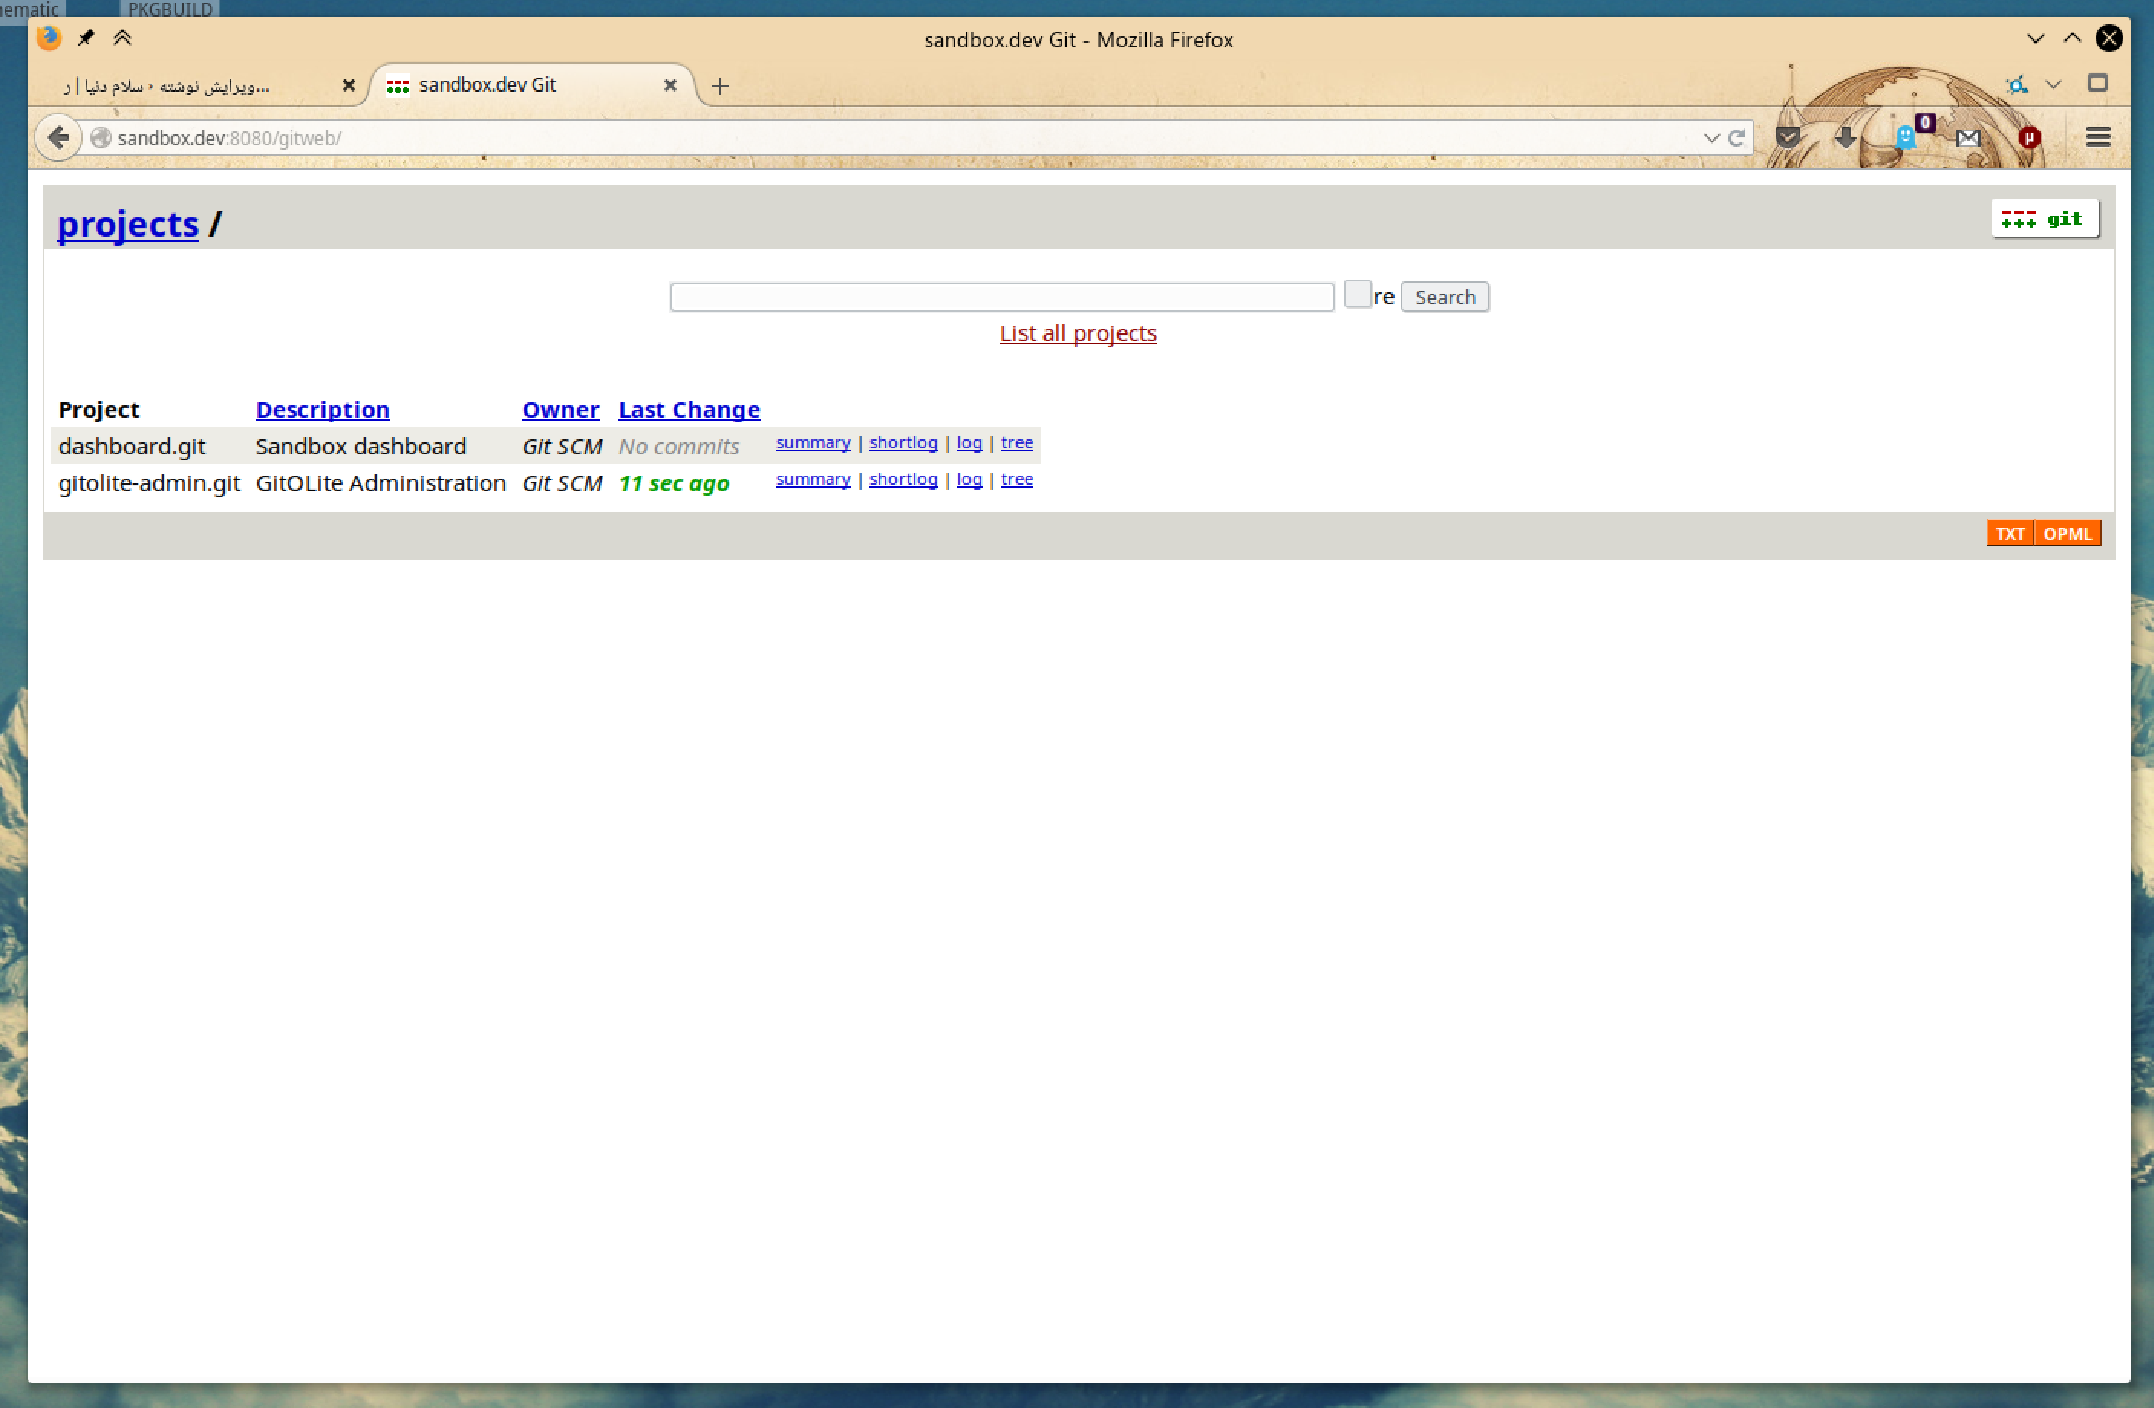
\includegraphics[width=.9\textwidth ,height=.65\textwidth]{Pic/GIT-WEB}
    \caption{ نمایی از گیت-وب 
        \lr{Gitweb page}   
    }
    \label{GIT-WEB}
\end{figure}

اما همانطور که می‌بینید؛ ابزار فوق از ظاهر مناسبی برخوردار نیست. برای آنکه ظاهر نرم‌افزار فوق بهبود یابد می‌توان از سبک‌های آماده‌ای که برای این منظور توسط کاربران در سطح وب نوشته شده است استفاده کنید. برای این‌کار مجددا به ترمینال مراجعه کنید. سپس به پوشه‌ای که در آن سبک های گیت‌وب قابل مشاهده است وارد خواهیم شد؛ ولی قبل از آن یک نسخه پشتیبان از سبک  و قالب فعلی تهیه می‌کنیم. 
\newline

\begin{latin}  
    \lstinputlisting[numbers=right,language=SH, framexleftmargin=5mm, frame=shadowbox,rulesepcolor=\color{White}]{Code/gitweb-bk.sh}
\end{latin}

سپس از طریق گیت، قالب مورد نظر را بارگیری می‌کنیم. این قالب در داخل گیت‌هاب قرار دارد؛ بنابر این آن را دریافت و  خروجی را با استفاده از «|»به پوشه «static» لوله‌کشی می‌کنیم.
\newline

\begin{latin}  
    \lstinputlisting[numbers=right,language=SH, framexleftmargin=5mm, frame=shadowbox,rulesepcolor=\color{White}]{Code/gitweb-theme.sh}
\end{latin}

حال اگر به همین آدرس 
\url{http://sandbox.dev:8080/gitweb/}
 مراجعه کنید با نمایی زیباتر از نرم‌افزار گیت‌وب مواجه خواهید شد. اگر از این قالب خوشتان نیامده است؛ می‌توانید قالب قبلی را از طریق تغییر نام پوشه «original» به «static» مجدد فعال کنید. نمای جدید در مرورگر فایرفاکس، در تصویر \ref{GIT-WEB-NEW} قابل مشاهده است.
 
 \begin{figure}
     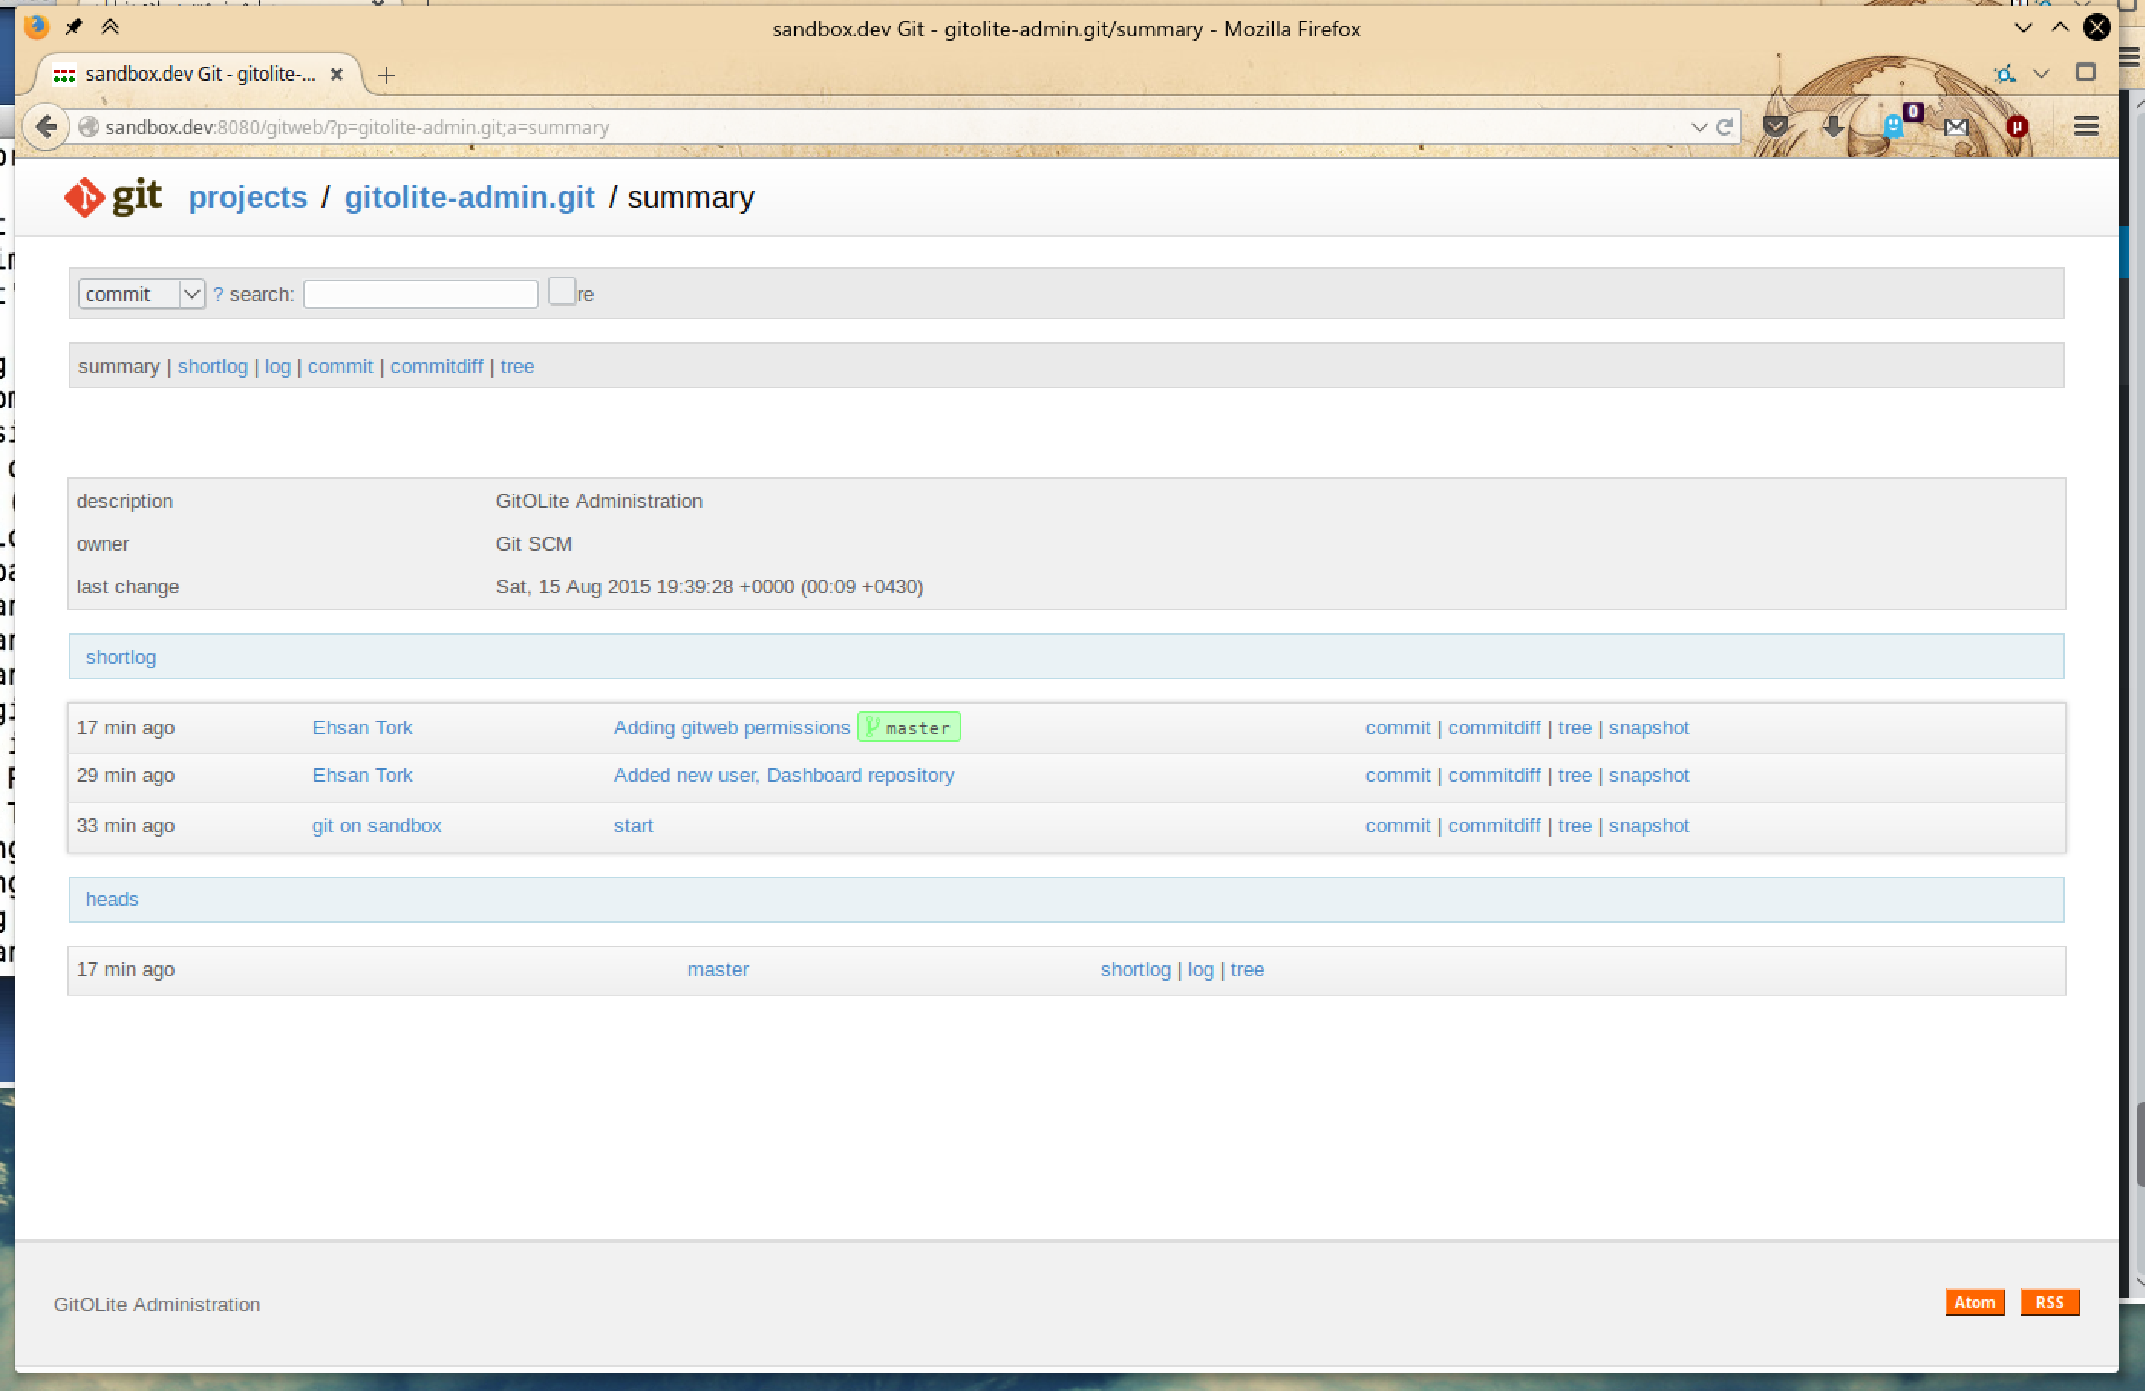
\includegraphics[width=.9\textwidth ,height=.60\textwidth]{Pic/GIT-WEB-NEW}
     \caption{ نمایی از سبک و قالب جدید گیت-وب 
         \lr{Gitweb new Theme}   
        }
        \label{GIT-WEB-NEW}
    \end{figure}

اگر تغییر احساس نکردید؛ صفحه را با کلیدهای 
\path{«CTRL + F8»}
، مجددا تازه سازی کنید. بعد از مشاهده صفحه فوق به شکل مناسب و زیبا، تقریبا آموزش نصب و تنظیم گیت‌وب به پایان رسیده‌است؛ با این حال آموزش نصب و تنظیم و چگونگی استفاده از نرم‌افزار «etckeeper» را نیز در قسمت بعدی بررسی خواهیم کرد. این ابزار جهت به‌هنگام‌سازی و همگام‌سازی تنظیمات سیستم توسط گیت به کار می‌رود.

استفاده از گیت و آموزش نحوه استفاده از آن برای دسترسی به سندباکس از حوصله این مطلب خارج است و نمی‌توان تمامی مواردی را که در گیت وجود دارد را در یک مطلب کوتاه بررسی کرد. با این حال بنا به سیستم‌عامل مورد استفاده خود می‌توانید با استفاده از گیت به کنترل نسخه و مدیریت پروژه‌های خود بپردازید. اگر مخزن جدیدی را نیز مدنظر دارید؛ آن مخزنها را نیز همانند مخزن پیشخوان «Dashboard» در تنظیمات «gitolite-admin» درج کنید. برای دسترسی به مخزن خاص مثلا پیشخوان از آدرسی مانند آدرس زیر استفاده می‌شود.
\newline

\begin{latin}  
    \lstinputlisting[numbers=right,language=SH, framexleftmargin=5mm, frame=shadowbox,rulesepcolor=\color{White}]{Code/dash-git-url.txt}
\end{latin}

همچنین برای دسترسی به گیت در سیستم‌عامل مک و ویندوز می‌توانید از نرم‌افزار «SourceTree» استفاده کنید که یک واسط گرافیکی برای نرم‌افزار گیت به حساب می‌آید. \ref{GIT-GUI}

 \begin{figure}
 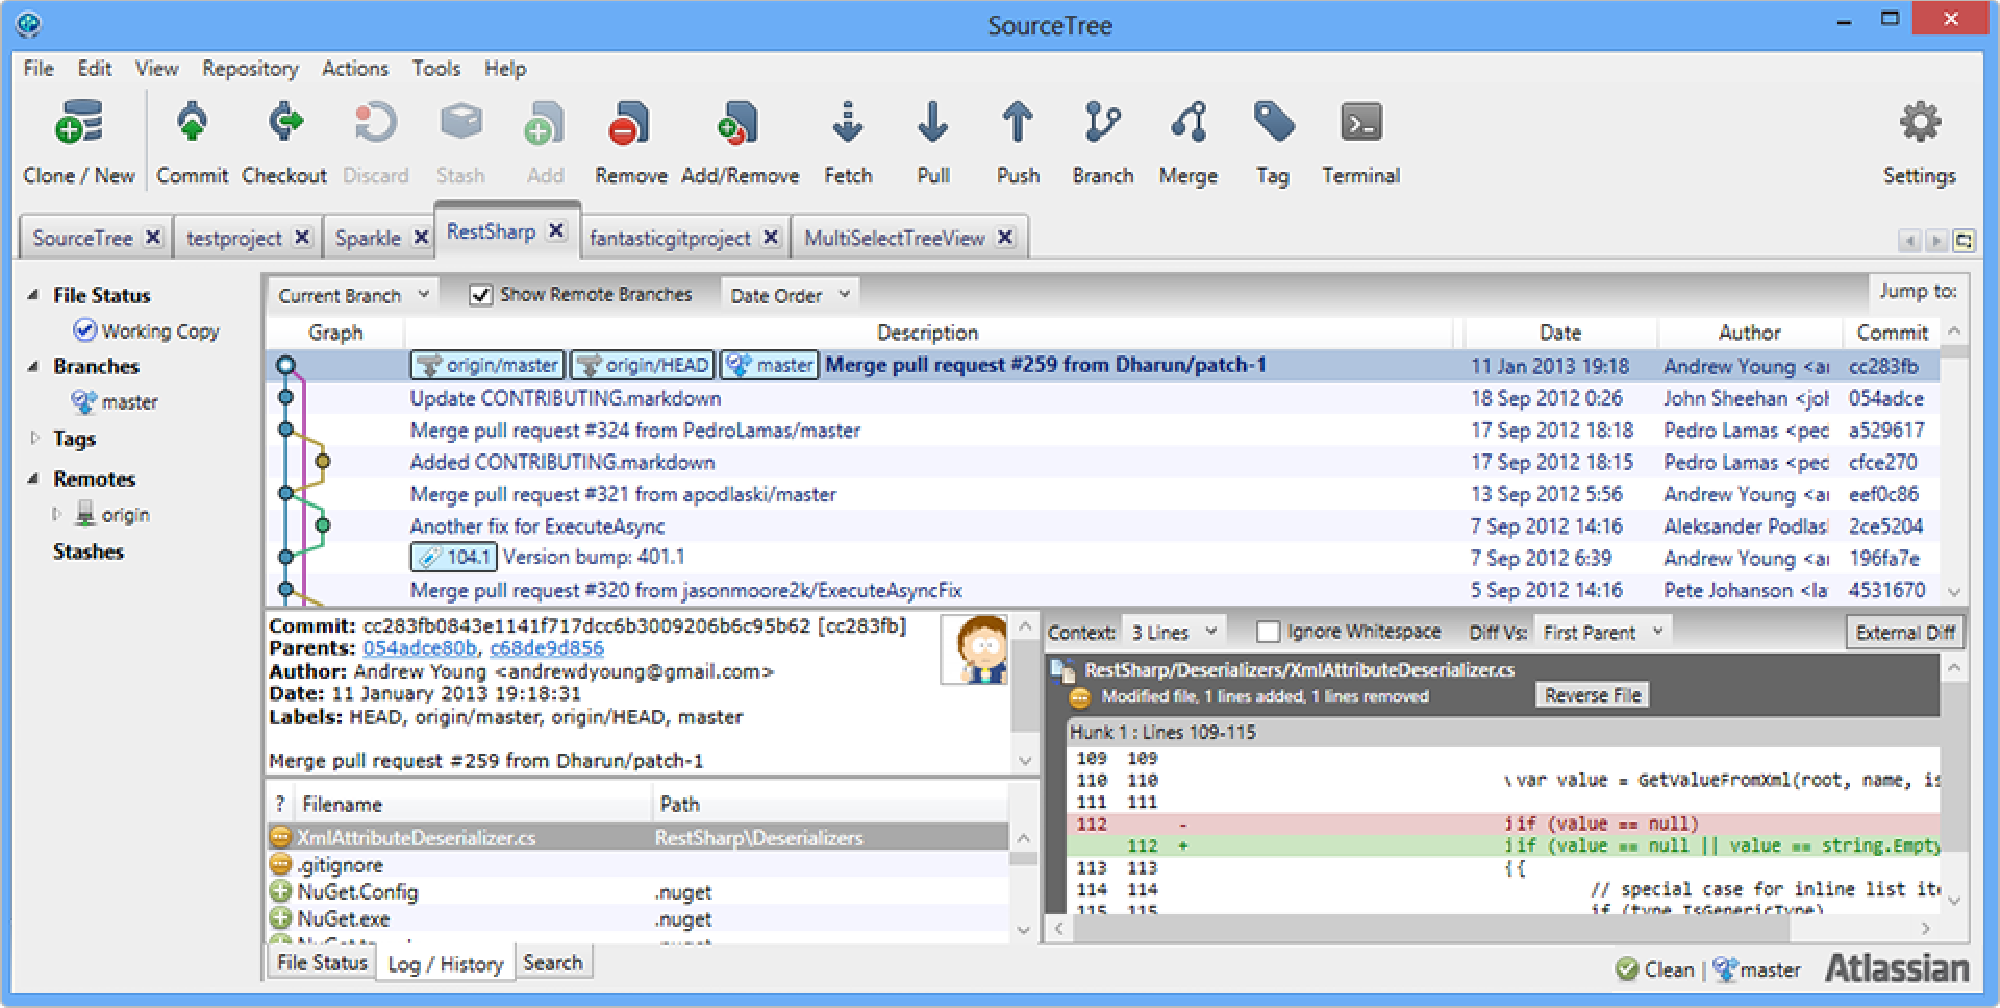
\includegraphics[width=.9\textwidth ,height=.50\textwidth]{Pic/GIT-GUI-WIN}
 \caption{ نمایی از واسط گرافیکی برای گیت 
 \lr{Git GUI Windows 8.0 - }   
  }
\label{GIT-GUI}
\end{figure}